\documentclass{article}

\usepackage[margin=1in]{geometry}
\usepackage{multicol}
\usepackage{bookmark}
\usepackage{adjustbox}
\usepackage{mathtools}
\usepackage{amsmath}
\usepackage{amssymb}
\usepackage{amsthm}
\usepackage{amsfonts}
\usepackage{algorithmic}

\usepackage{pgfplots}
\pgfplotsset{compat=1.16}
\usepackage{tikz}
\usetikzlibrary{arrows, decorations.markings}
\usepackage{graphicx}
\usepackage{pst-solides3d}
\usepackage{xcolor}
\usepackage{hyperref}
\usepackage[cache=false]{minted}

\usepackage{fancyhdr}
\usepackage{caption}
\usepackage{soul}
\usepackage{cite}
\usepackage{textcomp}

\usepackage{wasysym}

% Sets and related operators
\newcommand{\nats}{\mathbb{N}}                   % Natural numbers
\newcommand{\pnats}{\mathbb{N}^+}                % Positive natural numbers (excluding 0)

\newcommand{\ints}{\mathbb{Z}}                   % Integers
\newcommand{\pints}{\mathbb{Z}^+}                % Positive integers
\newcommand{\nints}{\mathbb{Z}^-}                % Negative integers

\newcommand{\rats}{\mathbb{Q}}                   % Rational numbers
\newcommand{\prats}{\mathbb{Q}^+}                % Positive rational numbers
\newcommand{\nrats}{\mathbb{Q}^-}                % Negative rational numbers

\newcommand{\reals}{\mathbb{R}}                  % Real numbers
\newcommand{\preals}{\mathbb{R}^+}               % Positive real numbers
\newcommand{\nreals}{\mathbb{R}^-}               % Negative real numbers

\newcommand{\irrats}{\mathbb{I}}                 % Irrational numbers

\newcommand{\pset}{\mathcal{P}}                  % Powerset
\newcommand{\card}{\abs}                         % Cardinality
\newcommand{\topology}{\mathcal{T}}              % Topology
\newcommand{\basis}{\mathcal{B}}                 % Basis
\newcommand{\oldemptyset}{\emptyset}             % Old empty set
\renewcommand{\emptyset}{\varnothing}            % New and nice empty set

% Operators
\DeclarePairedDelimiter\abs{\lvert}{\rvert}      % Absolute value
\DeclarePairedDelimiter\ceil{\lceil}{\rceil}     % Ceiling
\DeclarePairedDelimiter\floor{\lfloor}{\rfloor}  % Floor

% Other
\newcommand{\rarr}{\rightarrow}                  % Leftarrow
\newcommand{\larr}{\leftarrow}                   % Rightarrow (equivalent to \to)
\newcommand\und[1]{\underline{\smash{#1}}}       % Nice-looking underline
\renewcommand{\headrulewidth}{0.5pt}             % Header rule width
\renewcommand{\footrulewidth}{0pt}               % Footer rule width
\renewcommand{\baselinestretch}{1.5}             % Make the line spacing equal to 1.5

% Setting stuff
\setlength{\parindent}{0pt}                      % Remove indentations from paragraphs
\frenchspacing                                   % Sometimes latex creates unnecessarily large spaces after dots, this helps to avoid it (puts single spaces at the end of sentences)
\pagestyle{fancy}                                % This allows to do fancy headers and footers
\fancyhf{}                                       % No additional page numbering (or other stuff such as references)
\cfoot{\thepage}                                 % Display page number at the bottom in the center

\rhead{\footnotesize{\MakeUppercase{The Topology of Robotic Configuration and Motion Planning}}}


% Definition
\theoremstyle{definition}
\newtheorem*{definition}{Definition}


% Title
\title{The Topology of Robotic Configuration and Motion Planning\\
{\small \textsuperscript{*}The paper is written in the scope of the independent study course with Dr. Eric Westlund.}}

\author{David Oniani\\Luther College\\\href{mailto:oniada01@luther.edu}{oniada01@luther.edu}}

\date{January 30, 2019}


\begin{document}
\maketitle

%%%%%%%%%%%%%%%%%%%%%%%%%%%%%%%%%%%%%%%%%%%%%%%%%%%%%%%%%%%%%%%%%%%%%%%%%%%%%%%%%%%%%%%%%%%%%%%%%%%%

\begin{abstract}
\noindent This paper explores the topological approach to the problem
of robot motion planning. Particularly, we will discuss
the safe way to coordinate automated guided vehicles or AGVs.
AGVs are mobile robots which are used extensively in manufacturing
facilities. Since these robots are costly and cannot tolerate collisions,
one of the biggest challenges in designing such facility is setting up
mobile robot routes to achieve the safe and efficient coordination of robots.
The tools and concepts of topology are naturally employed in this planning
process. This paper follows the bottom-up approach by first introducing
concepts and then building up on these ideas. It does not assume any background
in topology nor in robotics. It is therefore accessible to most undergraduate
mathematics students with the knowledge of set theory.
\end{abstract}

%%%%%%%%%%%%%%%%%%%%%%%%%%%%%%%%%%%%%%%%%%%%%%%%%%%%%%%%%%%%%%%%%%%%%%%%%%%%%%%%%%%%%%%%%%%%%%%%%%%%

\section*{\centering Configuration Spaces}
We shall start by introducing the notion of configuration spaces.
The idea of configuration spaces come from physics. In classical mechanics,
the configuration space is the vector space defined by the generalized
coordinates (coordinates that describe the configuration of the physical system).
Put it simply, the configuration space is the set of all possible states that
could exist in the physical system. For instance, the configuration space of some
particle in the room is the set of all points/states of the type $(x, y, z)$ where
$x, y$ and $z$ are the coordinates bounded by the room. If the room is a $3 \times 3 \times 3$
cube then we define the configuration space of the particle by
$$C^3(\text{room}) = \{(x, y, z) \mid 0 \leq x, y, z \leq 3\}.$$
In other words, the configuration space of the particle, is all of $3 \times 3 \times 3$ cube
(this example obviously assumes that the particle is allowed to move freely in the room).
The configuration space of the same particle in a spherical room, however, would be the set of all
points that are in a sphere. More formally, we call the the states of the particle configurations
and the space of all configurations - a configuration space.

\bigskip

It appears that the physical notion of configuration spaces is very much connected to that of mathematics.
In fact, the idea is the same but rather generalized. To better understand configuration spaces, let us
first go through several \textit{classic} examples.

\bigskip

\cite{1} Consider a planar system where we have a rod with a fixed end that can rotate freely. Then it is
easy to see that the space of all possible configurations of the rotating rod is a circle.

\begin{figure}[H]
\centering
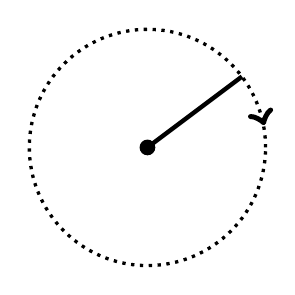
\begin{tikzpicture}
    % Circle
    \draw[
        black,
        very thick,
        dotted,
        decoration={markings, mark=at position 0.05 with {\arrow[draw=black, line width=2.25pt]{<}}},
        postaction={decorate}
        ]
        (2, 2) circle (1.5);

    % Rotating rod
    \draw[black, ultra thick] (2, 2) -- (3.2, 2.9);

    % Fixed endpoint
    \fill (2, 2) circle (0.1);
\end{tikzpicture}
\caption*{Circle obtained by the rotational motion of the rod.}
\end{figure}

In other words, as the rod rotates, it creates the circle around itself
with the radius equal to the length of the rod. This configuration space
is also referred to as $S^1$.

\bigskip

\cite{2} On the other hand, the configuration space of the two-rod
system in 3D space where one rod is fixed and the other one is attached to it (also known as a 2R robot)
is a torus. This space is also known as $S^1 \times S^1$ configuration space.

\begin{figure}[H]
\centering
\includegraphics[width=4cm, height=4cm]{two-rod-system}
\caption*{A two-rod system.}
\end{figure}

We already know that a rod with fixed end generates a circle. In this case,
we have two rods: one attached to the ground and the other one attached to the end
of the first one. Then obviously both of the rods can go through a full circle
of states and therefore, create a configuration space which geometrically represents a torus.

\begin{figure}[H]
    \centering
    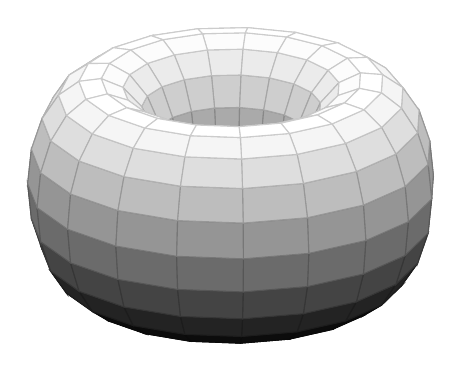
\begin{tikzpicture}
        \begin{axis}[hide axis]
           \addplot3[
               surf,
               colormap/blackwhite,
               samples=20,
               domain=0:2*pi,
               y domain=0:2*pi,
               z buffer=sort
             ]
             ( {(2 + cos(deg(x))) * cos(deg(y + pi/2))}, 
               {(2 + cos(deg(x))) * sin(deg(y + pi/2))}, 
               {sin(deg(x))}
             );
        \end{axis}
      \end{tikzpicture}
    \caption*{A torus obtained by the motion of two-rod system.}
\end{figure}

As of now, this is all we need to know about the configuration spaces.
This idea will be very useful once we learn more about other topological concepts.

%%%%%%%%%%%%%%%%%%%%%%%%%%%%%%%%%%%%%%%%%%%%%%%%%%%%%%%%%%%%%%%%%%%%%%%%%%%%%%%%%%%%%%%%%%%%%%%%%%%%

\section*{\centering Topological Spaces}
The fundamental idea in topology is that of a topological space.
We will use this idea to then introduce and define other important concepts.

\begin{definition}
\cite{3} A \textit{\textbf{topology}} on a set $X$ is a collection $\topology$ of subsets of $X$ having
the following properties:

\begin{itemize}
\item[(1)]
$\emptyset$ and $X$ are in $\topology$.

\item[(2)]
The union of the elements of any subcollection of $\topology$ is in $\topology$.

\item[(3)]
The intersection of the elements of any finite subcollection of $\topology$ is in $\topology$.
\end{itemize}

A set $X$ for which a topology $\topology$ has been specified is called a \textit{\textbf{topological space}}.
\end{definition}

Let us first look at some examples. Consider a set $X = \{a, b, c\}$.
Then we can define a topology on $X$ by $\topology = \{\emptyset, \{a, b, c\}, \{a, b\}, \{c\}\}$.
Observe that $\emptyset, X \in \topology$ therefore the first criterion is satisfied.
It is easy to see that arbitrary unions will be in $\topology$ since the only ``interesting''
case is when we consider $\{a, b\}$ and $\{c\}$, but in this case $\{a, b\} \cup \{c\} = \{a, b, c\} \in \topology$.
This satisfies the second requirement. Finally, any arbitrary intersection of the finite subcollections of $\topology$
is also in $\topology$ and therefore, we conclude that $\topology$ is indeed a topology on $X$.
Hence, $X$ is a topological space (note that, properly speaking, a topological space is an ordered pair $(X, \topology)$,
but we often omit mentioning $\topology$ and say that $X$ is a topological space).

\bigskip

At this point, you might have already noticed that one could always define more than one topology
for a given set. In the previous example, sets $\pset{(x)}$ (powerset of $x$) and $\{\emptyset, X\}$
are also topologies on $X$ called discrete and indiscrete topologies. In fact, for any set $X$,
$\pset{(x)}$ and $\{\emptyset, X\}$ will always be two distinct topologies on $X$.

\bigskip

We will now get acquainted with the notion of the \textit{open set}.

\begin{definition}
\cite{4}  If $X$ is a topological space with topology $\topology$, we say that a subset $U$ of $X$ is an
\textbf{open set} of $X$ if $U$ belongs to the collection $\topology$.
\end{definition}

Consider our topology $\topology = \{\emptyset, \{a, b, c\}, \{a, b\}, \{c\}\}$ on the topological space $X = \{a, b, c\}$.
Then notice that $\emptyset, \{a, b, c\}, \{a, b\}, \{c\} \in \topology$ and therefore, all are open sets.

%%%%%%%%%%%%%%%%%%%%%%%%%%%%%%%%%%%%%%%%%%%%%%%%%%%%%%%%%%%%%%%%%%%%%%%%%%%%%%%%%%%%%%%%%%%%%%%%%%%%

\section*{\centering Continuous Functions and Homeomorphisms}
The notion of continuous functions is familiar to most high-school students.
Most people associate them with a nice-looking monotonically increasing or decreasing
functions with no leaps or jumps. There are several definitions for a function continuity.
Here is the calculus definition.

\begin{definition}
\cite{5} A function $f(x)$ is continuous at a point $x = c$ if and only if it meets the following
three conditions:\\
1. $f(c)$ exists ($c$ lies in the domain of $f$).\\
2. $\lim_{x \to c}f(x)$ exists ($f$ has a limit as $x \to c$).\\
3. $\lim_{x \to c}f(x) = f(c)$ (the limit equals to the function value).
\end{definition}

In topology we cannot really use this definition since the definition assumes
that one could take a limit of the function. This, however, is sometimes very difficult or nearly impossible
when considering functions defined over more abstract sets such as the configuration space
of AGV. Now, we shall introduce more general notion of continuity.

\begin{definition}
\cite{6} Let $X$ and $Y$ be topological spaces. A function $f : X \to Y$ is said to be \textbf{continuous} if
for each open subset $V$ of $Y$, the set $f^{-1}(V)$ is an open subset of $X$.
\end{definition}

It is important to note that in this definition $f^{-1}(V)$ does not refer to the inverse of the function.
Therefore, we are not assuming that $f : X \rarr Y$ is a bijection. $f^{-1}(V)$ refers to the preimage of the function.
In other words, the function $f : X \to Y$ over two topological spaces $X$ and $Y$ is continuous if and only if every open
set in the image is mapped by an open set from a preimage.

\bigskip

This is the case where the visualization might be useful to see how the definition of continuous functions really works.
Consider a continuous function $f : X \to Y$ where $X$ and $Y$ are topological spaces with topologies $\topology_X$ and $\topology_Y$.

\begin{figure}[H]
    \centering
    \includegraphics[width=7.5cm, height=4cm]{continuous-function}
    \caption*{A continuous function $f : X \to Y$.}
\end{figure}

In the figure above, the big blobs $X$ and $Y$ are topological spaces and smaller blobs $\topology_X$
and $\topology_Y$ are the topologies on $X$ and $Y$ correspondigly. By the definition, the elements in $\topology_X$
or $\topology_Y$ are open sets. Then notice that the function $f : X \to Y$ shown above is continuous. All the points
which are in $\topology_Y$ have a preimage in $\topology_X$. Note that there are points in $Y$ that do not have a preimage
in $\topology_X$, but it has no importance to continuity of $f$ since it must be open sets in $Y$ (not just any set) that must
have an open preimage.

\bigskip

The function below, however, is not continuous as there is one point that is not in $\topology_X$
but maps to a point in $\topology_Y$ (it is highlighted with the red arrow).

\begin{figure}[H]
    \centering
    \includegraphics[width=7.5cm, height=4cm]{discontinuous-function}
    \caption*{A discontinuous function $f : X \to Y$.}
\end{figure}

\bigskip

Now that we are familiar with the notion of continuous functions, we shall introduce a new idea, that of homeomorphisms.

\begin{definition}
\cite{7} Let $X$ and $Y$ be topological spaces; let $f : X \to Y$ be a bijection. If both the function $f$
and the inverse function
$$f^{-1} : Y \to X$$
are continuous, then $f$ is called a homeomorphism.
\end{definition}

As one delves deeper in topology, this definition is then taken further and two objects are said to be homeomorphic if
one could be obtained by the continuous deformation of the other. We may not use this notion further in the paper yet,
it is a helpful way to think about homeomorphisms.

%%%%%%%%%%%%%%%%%%%%%%%%%%%%%%%%%%%%%%%%%%%%%%%%%%%%%%%%%%%%%%%%%%%%%%%%%%%%%%%%%%%%%%%%%%%%%%%%%%%%

\section*{\centering Connectedness and Path Connectedness}
One of the important ideas in topology is that of connectedness.
This idea is used extensively in various other fields of mathematics such as graph theory and knot theory.
Let us first define connectedness.

\begin{definition}
\cite{8} Let $X$ be a topological space. A \textbf{separation} of $X$ is a pair $U, V$ of disjoint
nonempty open subsets of $X$ whose union is $X$. The space $X$ is said to be \textbf{connected}
if there does not exist a separation of $X$.
\end{definition}

Consider a topological space $X = \{a, b, c\}$ with a topology $\topology = \{\emptyset, \{a, b, c\}, \{a, b\}, \{c\}\}$.
Then it is easy to see that $X$ is a disconnected space. Sets $\{a, b\}$ and $\{c\}$ are open since $\{a, b\}, \{c\} \in \topology$.
Besides, $\{a, b\} \cap \{c\} = \emptyset$ and $\{a, b\} \cup \{c\} = \{a, b, c\} = X$.
Hence, $U = \{a, b\}$ and $V = \{c\}$ is a pair of disjoint open subsets of $X$ whose union is $X$
and therefore $U, V$ is a separation of $X$. This means that $X$ is a disconnected space.

\bigskip

On the other hand, a topological space $Y = \{a, b\}$ with a topology $\topology = \{\emptyset, \{a, b\}, \{a\}\}$
is connected as there is no pair of disjoint nonempty open subsets of $Y$ such that their union is $Y$.
In other words $Y$ has no separation. Note that $\emptyset \cup \{a, b\} = \{a, b\} = Y$, but it must be \und{nonempty}
sets whose union is $Y$. Therefore, $\emptyset, \{a, b\}$ is not a separation of $Y$.

\bigskip

Knowing what it means for a topological space to be connected, we can now introduce the notion
of path connectedness.

\begin{definition}
\cite{9} Given points $x$ and $y$ of the space $X$, a \textbf{path} in $X$ from $x$ to $y$ is a 
continuous map $f : [a, b] \to X$ of some closed interval in the real line into $X$, such
that $f(a) = x$ and $f(b) = y$. A space $X$ is said to be \textit{\textbf{path connected}} if every pair of
points of $X$ can be joined by a path in $X$.
\end{definition}

Path connected spaces are certainly related to the connected spaces.
In fact, one could easily verify that path connectedness implies connectedness.
Therefore, every path-connected space is connected.

%%%%%%%%%%%%%%%%%%%%%%%%%%%%%%%%%%%%%%%%%%%%%%%%%%%%%%%%%%%%%%%%%%%%%%%%%%%%%%%%%%%%%%%%%%%%%%%%%%%%

\section*{\centering Configuration Spaces Revisited - Robotic Configurations}
In previous sections, we went through what is called a configuration space.
Yet, we did not have a precise definition for it since it varies from field to field.
Let us now define what a configuration space means in the robotics context.

\begin{definition}
\cite{10} A \textit{\textbf{configuration}} of a robot is a specification of the position of all points of a robot.
The \textit{\textbf{configuration space}} of a robot is the space of all configurations of a robot.
\end{definition}

Suppose that we have a robot $R$ that can move freely on a line $L$. Then we can model the robot as
a point with a coordinate $x_R$. The configuration space for this robot is

$$C^1(L) = \{x_R \mid x_R \in L\} = L = L^1.$$

with every point in the room being a unique configuration of the robot.
The dimension of $C$ (in this case 1), is also called \textit{\textbf{degree(s) of freedom}}.
In this case, the configuration space $C$ has 1 degree of freedom.

\bigskip

What if we had 2 robots (say $R_1$ and $R_2$) that can move freely?
Then the configuration space would be $C^2$ which can be represented as a set
$$C^2(L) = \{(x_{R_1}, x_{R_2}) \mid x_{R_1}, x_{R_2} \in L\} = L \times L = L^2.$$

In general, the configuration space for $N$ robots $R_1, R_2, \dots, R_N$ that can move freely on a line $L$ is

$$C^N(L) = \{(x_{R_1}, x_{R_2}, \dots, x_{R_N}) \mid x_{R_1}, x_{R_2}, \dots, x_{R_N} \in L\} = \underbrace{L \times L \times \dots \dots L}_{N \ \text{times}} = L^N$$

In fact, we could generalize this notion even further. Instead of considering
$N$ robots moving on a line $L$, suppose that we have $N$ robots moving on some
$K$-dimensional space $L^K$. Then the configuration for each of the robots will
be a $K$-tuple and the configuration space of all $N$ robots will be a set consisting
of $N$ number of $K$-tuples. Therefore, we have

$$C(L^K) = \{(x_{R_{1, 1}}, x_{R_{2, 1}}, \dots, x_{R_{N, 1}}), \dots, (x_{R_{2, K}}, \dots, x_{R_{N, K}}) \mid x_{R_{1, 1}}, \dots, x_{R_{N, 1}}, \dots, x_{R_{1, K}}, \dots, x_{R_{N, K}} \in L^K\}.$$

where $(x_{R_{1, 1}}, x_{R_{2, 1}}, \dots, x_{R_{N, 1}})$ one configuration (with $x_{R_{1, 1}}$ being the configuration of the first robot, $x_{R_{2, 1}}$ of the second robot etc.), $(x_{R_{1, 2}}, x_{R_{2, 2}}, \dots, x_{R_{N, 2}})$ is the other, and it goes all
the way up until $(x_{R_{1, K}}, x_{R_{2, K}}, \dots, x_{R_{N, K}})$.

%%%%%%%%%%%%%%%%%%%%%%%%%%%%%%%%%%%%%%%%%%%%%%%%%%%%%%%%%%%%%%%%%%%%%%%%%%%%%%%%%%%%%%%%%%%%%%%%%%%%

\section*{\centering Safe Robotic Configurations}
At this point, we have enough machinery to understand safe robotic configurations.
Let us model each robot with a point that moves through a topological space represeting
the robot routes in the factory.

\bigskip

Consider two robots $R_1$ and $R_2$ moving through the line represented by $L$ ($L$ is obviously a topological space).
Then the configuration space for these robots is
$$C = \{(x_{R_1}, x_{R_2}\} \mid x_{R_1}, x_{R_2} \in L\} = L \times L = L^2.$$
The result here is somewhat natural. If we have one robot moving on a line, we have a configuration
space $L$. If there are two robots, the configuration changes from a single point to a 2-tuple ($(x_A, x_B)$ in the case)
which yields a configuration space equal to that of $L^2$.

\bigskip

Now, since $x_{R_1}$ and $x_{R_2}$ represent the coordinates of the robots, we cannot allow them to be the same.
In other words, if $x_{R_1} = x_{R_2}$, we have a collision. We therefore modify our configuration space $C$
to eliminate all the configurations where $x_{R_1} = x_{R_2}$. Let us call this new configuration space $SC$
(safe configuration) with
$$SC = \{(x_{R_1}, x_{R_2}) \mid x_{R_1}, x_{R_2} \in \reals, x_{R_1} \neq x_{R_2}\}.$$

\bigskip

It is really helpful to think about this configuration space geometrically.
Particularly, let's think about this space as a small chunk of the $XOY$ coordinate system.
To do this, we will need to do some transformations. Since $L$ is a line we might as well
represent it a closed interval $L = [0, a]$ where $a \in \reals$. Now we can say that both
robots $R_1$ and $R_2$ are moving through the interval $[0, a]$.
Let us consider the motion of $R_1$ and $R_2$ independently. To do this, we make a copy
of the interval $[0, a]$, put one interval as an $X$ axis and the other one as the $Y$ axis.

\begin{figure}[H]
\centering
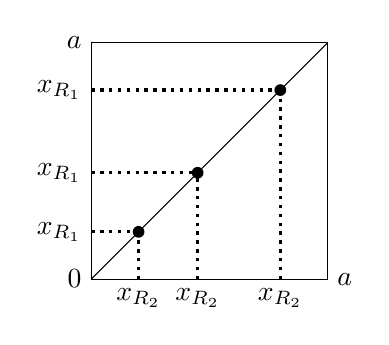
\begin{tikzpicture}[scale=1.5]
    % Draw the square
    \draw (0, 0) -- (2, 0) -- (2, 2) -- (0, 2) -- (0, 0);
    % Points
    \node [left] at (0, 2) {$a$};
    \node [right] at (2, 0) {$a$};
    \node [left] at (0, 0) {$0$};
    % 0.4, 0.4
    \node [left] at (0, 0.4) {$x_{R_1}$};
    \node [below] at (0.4, 0) {$x_{R_2}$};
    \node at (0.4, 0.4) [circle, fill, inner sep=1.5pt]{};
    % 0.9, 0.9
    \node [left] at (0, 0.9) {$x_{R_1}$};
    \node [below] at (0.9, 0) {$x_{R_2}$};
    \node at (0.9, 0.9) [circle, fill, inner sep=1.5pt]{};
    % 1.6, 1.6
    \node [left] at (0, 1.6) {$x_{R_1}$};
    \node [below] at (1.6, 0) {$x_{R_2}$};
    \node at (1.6, 1.6) [circle, fill, inner sep=1.5pt]{};
    % Lines
    \draw (0, 0) -- (2, 2);
    % 0.4, 0.4
    \draw [dotted, very thick] (0, 0.4) -- (0.4, 0.4);
    \draw [dotted, very thick] (0.4, 0) -- (0.4, 0.4);
    % 0.9, 0.9
    \draw [dotted, very thick] (0, 0.9) -- (0.9, 0.9);
    \draw [dotted, very thick] (0.9, 0) -- (0.9, 0.9);
    % 1.6, 1.6
    \draw [dotted, very thick] (0, 1.6) -- (1.6, 1.6);
    \draw [dotted, very thick] (1.6, 0) -- (1.6, 1.6);
\end{tikzpicture}
\end{figure}

From the picture above, it is easy to see that the points where $x_{R_1} = x_{R_2}$
are the points on the \textbf{diagonal} of the square bounded by interval $[0, a]$ on $X$ axis
and its copy on the $Y$ axis. This diagonal is denoted by $\Delta$. Then we can simply
say that

$$SC = C - \Delta.$$

In the general case with $N$ robots and the topological space $X$, it is easy to see that
$$SC^N = \underbrace{X \times X \times \dots \times X}_{N \ \text{times}} - \Delta \ \text{where} \ \Delta = \{(x_1, x_2, \dots, x_N) \mid x_i = x_j \ \text{for some} \ i \neq j\}$$

We are basically taking the product of $N$ copies of $X$ because we have $N$ robots
and we have to account for the position of each robot independent. Every configuration
in this configuration space will look like $(x_1, x_2, \dots x_N)$ and we eliminate each
configuration for which there exists $x_i$ and $x_j$ such that $x_i = x_j$ with $i \neq j$.
This means that we do not allow any two robots to have the same coordinates in any configuration.

%%%%%%%%%%%%%%%%%%%%%%%%%%%%%%%%%%%%%%%%%%%%%%%%%%%%%%%%%%%%%%%%%%%%%%%%%%%%%%%%%%%%%%%%%%%%%%%%%%%%

\section*{\centering Safe Robotic Relocations}
Now that we know about safe robotic configurations, let us model the relocation
of $n$ robots in the space $X$. To do this, we need to use a path in $SC^n(X)$.
Suppose that initially the robots had the configuration $(I_1, I_2, \dots, I_n)$
where $I_K$ is the initial position of the $K$-th robot. Then we define what is
called the \textbf{relocation} of these $n$ robots.

\begin{definition}
\cite{11} We define a \textit{\textbf{relocation}} of the $n$ robots from the initial configuration
$I = (I_1, \dots, I_n)$ to the finial configuration $F = (F_1, \dots, F_n)$ to be a path
$p : [0, 1] \to SC^n(X)$ such that $p(0) = I$ and $P(1) = F$.
\end{definition}

Since the robots are mapped to the configuration in $SC^n(X)$, by the definition of $SC$,
there is no way that any two robots will occupy the same coordinate and therefore, the map
will ensure that there are no collisions.

\bigskip

We can now define \textbf{attainability} of configurations.

\begin{definition}
\cite{12} Given two configurations of the robots, $M = (M_1, \dots, M_n)$ and $N = (N_1, \dots, N_n)$,
we say that $N$ is \textit{\textbf{attainable}} from $M$ if there is a relocation of the robots
from $M$ to $N$.
\end{definition}

Now let's apply the definition of path connectedness that we covered a few chapter ago.
Notice that if the safe configuration space $SC^n(X)$ is path connected, then every configuration
is attainable from every other one and therefore, robots can move freely in the space.
In this case, we say that the robots are \textbf{freely transportable in} $X$.

\bigskip

Let's look at some examples. Consider two robots $R_1$ and $R_2$ on the line $L$ that we discussed previously.
We know that the safe configuration space for two robots is the square without the diagonal.

\begin{figure}[H]
    \centering
    \begin{tikzpicture}[scale=1.5]
        % Draw the square
        \draw (0, 0) -- (2, 0) -- (2, 2) -- (0, 2) -- (0, 0);
        % Points
        \node [left] at (0, 2) {$a$};
        \node [right] at (2, 0) {$a$};
        \node [left] at (0, 0) {$0$};
        % Lines
        \draw [dotted, very thick] (0, 0) -- (2, 2);
    \end{tikzpicture}
    \caption*{A safe configuration space for two robots moving on the line $L$.}
\end{figure}

Then notice that this safe configuration space is not path connected (recall that path connectedness
means that every pair of points of $SC$ can be joined by a path in $SC$). It is easy to show by taking
one point on the one side of the diagonal and the other one on the other side (note that these points
are really the configurations for the space). If one would connect these points, there would not be a
way to avoid intersection of the diagonal (a collision).

\begin{figure}[H]
    \centering
    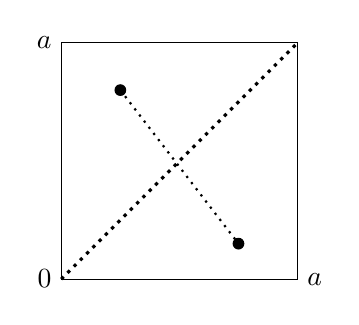
\begin{tikzpicture}[scale=1.5]
        % Draw the square
        \draw (0, 0) -- (2, 0) -- (2, 2) -- (0, 2) -- (0, 0);
        % Points
        \node [left] at (0, 2) {$a$};
        \node [right] at (2, 0) {$a$};
        \node [left] at (0, 0) {$0$};
        \node at (0.5, 1.6) [circle, fill, inner sep=1.5pt]{};
        \node at (1.5, 0.3) [circle, fill, inner sep=1.5pt]{};
        % Lines
        \draw [dotted, very thick] (0, 0) -- (2, 2);
        \draw [dotted, thick] (0.5, 1.6) -- (1.5, 0.3);
    \end{tikzpicture}
    \caption*{Attempt to connect two points from one side of diagonal to the other.}
\end{figure}

Then, by the definition of free transportability, $R_1$ and $R_2$ are not freely
transportable in $L$.

%%%%%%%%%%%%%%%%%%%%%%%%%%%%%%%%%%%%%%%%%%%%%%%%%%%%%%%%%%%%%%%%%%%%%%%%%%%%%%%%%%%%%%%%%%%%%%%%%%%%

\begin{center}
\begin{thebibliography}{00}
    \bibitem{1} Adams C. and Fransoza R., ``Introduction to Topology'' (2008), p. 105.
    \bibitem{2} Adams C. and Fransoza R., ``Introduction to Topology'' (2008), pp. 105 -- 106.
    \bibitem{3} Munkres J. R., ``Topology'' (2000), Second Edition, Upper Saddle River, NJ: Prentice Hall., p. 76
    \bibitem{4} Munkres J. R., ``Topology'' (2000), Second Edition, Upper Saddle River, NJ: Prentice Hall., p. 76
    \bibitem{5} Thomas G. B., ``Thomas' Calculus" (2010), Thirteenth Edition, p. 77
    \bibitem{6} Munkres J. R., ``Topology'' (2000), Second Edition, Upper Saddle River, NJ: Prentice Hall., p. 102
    \bibitem{7} Munkres J. R., ``Topology'' (2000), Second Edition, Upper Saddle River, NJ: Prentice Hall., p. 105
    \bibitem{8} Munkres J. R., ``Topology'' (2000), Second Edition, Upper Saddle River, NJ: Prentice Hall., p. 148
    \bibitem{9} Munkres J. R., ``Topology'' (2000), Second Edition, Upper Saddle River, NJ: Prentice Hall., p. 155
    \bibitem{10} Lynch K. and Park F., ``Modern Robotics: Mechanics, Planning, and Control'', Chapter 2.1,\\\href{https://youtube.com/watch?v=z29hYlagOYM}{https://youtube.com/watch?v=z29hYlagOYM}.
    \bibitem{11} Adams C. and Fransoza R., ``Introduction to Topology'' (2008), p. 199
    \bibitem{12} Adams C. and Fransoza R., ``Introduction to Topology'' (2008), p. 199
\end{thebibliography}
\end{center}

\end{document}
